
\documentclass[]{standalone}


\usepackage{tikz}
\usetikzlibrary{calc, patterns}

\newlength{\hatchspread}
\newlength{\hatchthickness}
\newlength{\hatchshift}
\newcommand{\hatchcolor}{}
% declaring the keys in tikz
\tikzset{hatchspread/.code={\setlength{\hatchspread}{#1}},
         hatchthickness/.code={\setlength{\hatchthickness}{#1}},
         hatchshift/.code={\setlength{\hatchshift}{#1}},% must be >= 0
         hatchcolor/.code={\renewcommand{\hatchcolor}{#1}}}
% setting the default values
\tikzset{hatchspread=3pt,
         hatchthickness=0.4pt,
         hatchshift=0pt,% must be >= 0
         hatchcolor=black}
% declaring the pattern
\pgfdeclarepatternformonly[\hatchspread,\hatchthickness,\hatchshift,\hatchcolor]% variables
   {custom north west lines}% name
   {\pgfqpoint{\dimexpr-2\hatchthickness}{\dimexpr-2\hatchthickness}}% lower left corner
   {\pgfqpoint{\dimexpr\hatchspread+2\hatchthickness}{\dimexpr\hatchspread+2\hatchthickness}}% upper right corner
   {\pgfqpoint{\dimexpr\hatchspread}{\dimexpr\hatchspread}}% tile size
   {% shape description
    \pgfsetlinewidth{\hatchthickness}
    \pgfpathmoveto{\pgfqpoint{0pt}{\dimexpr\hatchspread+\hatchshift}}
    \pgfpathlineto{\pgfqpoint{\dimexpr\hatchspread+0.15pt+\hatchshift}{-0.15pt}}
    \ifdim \hatchshift > 0pt
      \pgfpathmoveto{\pgfqpoint{0pt}{\hatchshift}}
      \pgfpathlineto{\pgfqpoint{\dimexpr0.15pt+\hatchshift}{-0.15pt}}
    \fi
    \pgfsetstrokecolor{\hatchcolor}
    \pgfusepath{stroke}
   }



\usepackage[nomessages]{fp}

\usepackage{graphicx}

\begin{document}

\sffamily

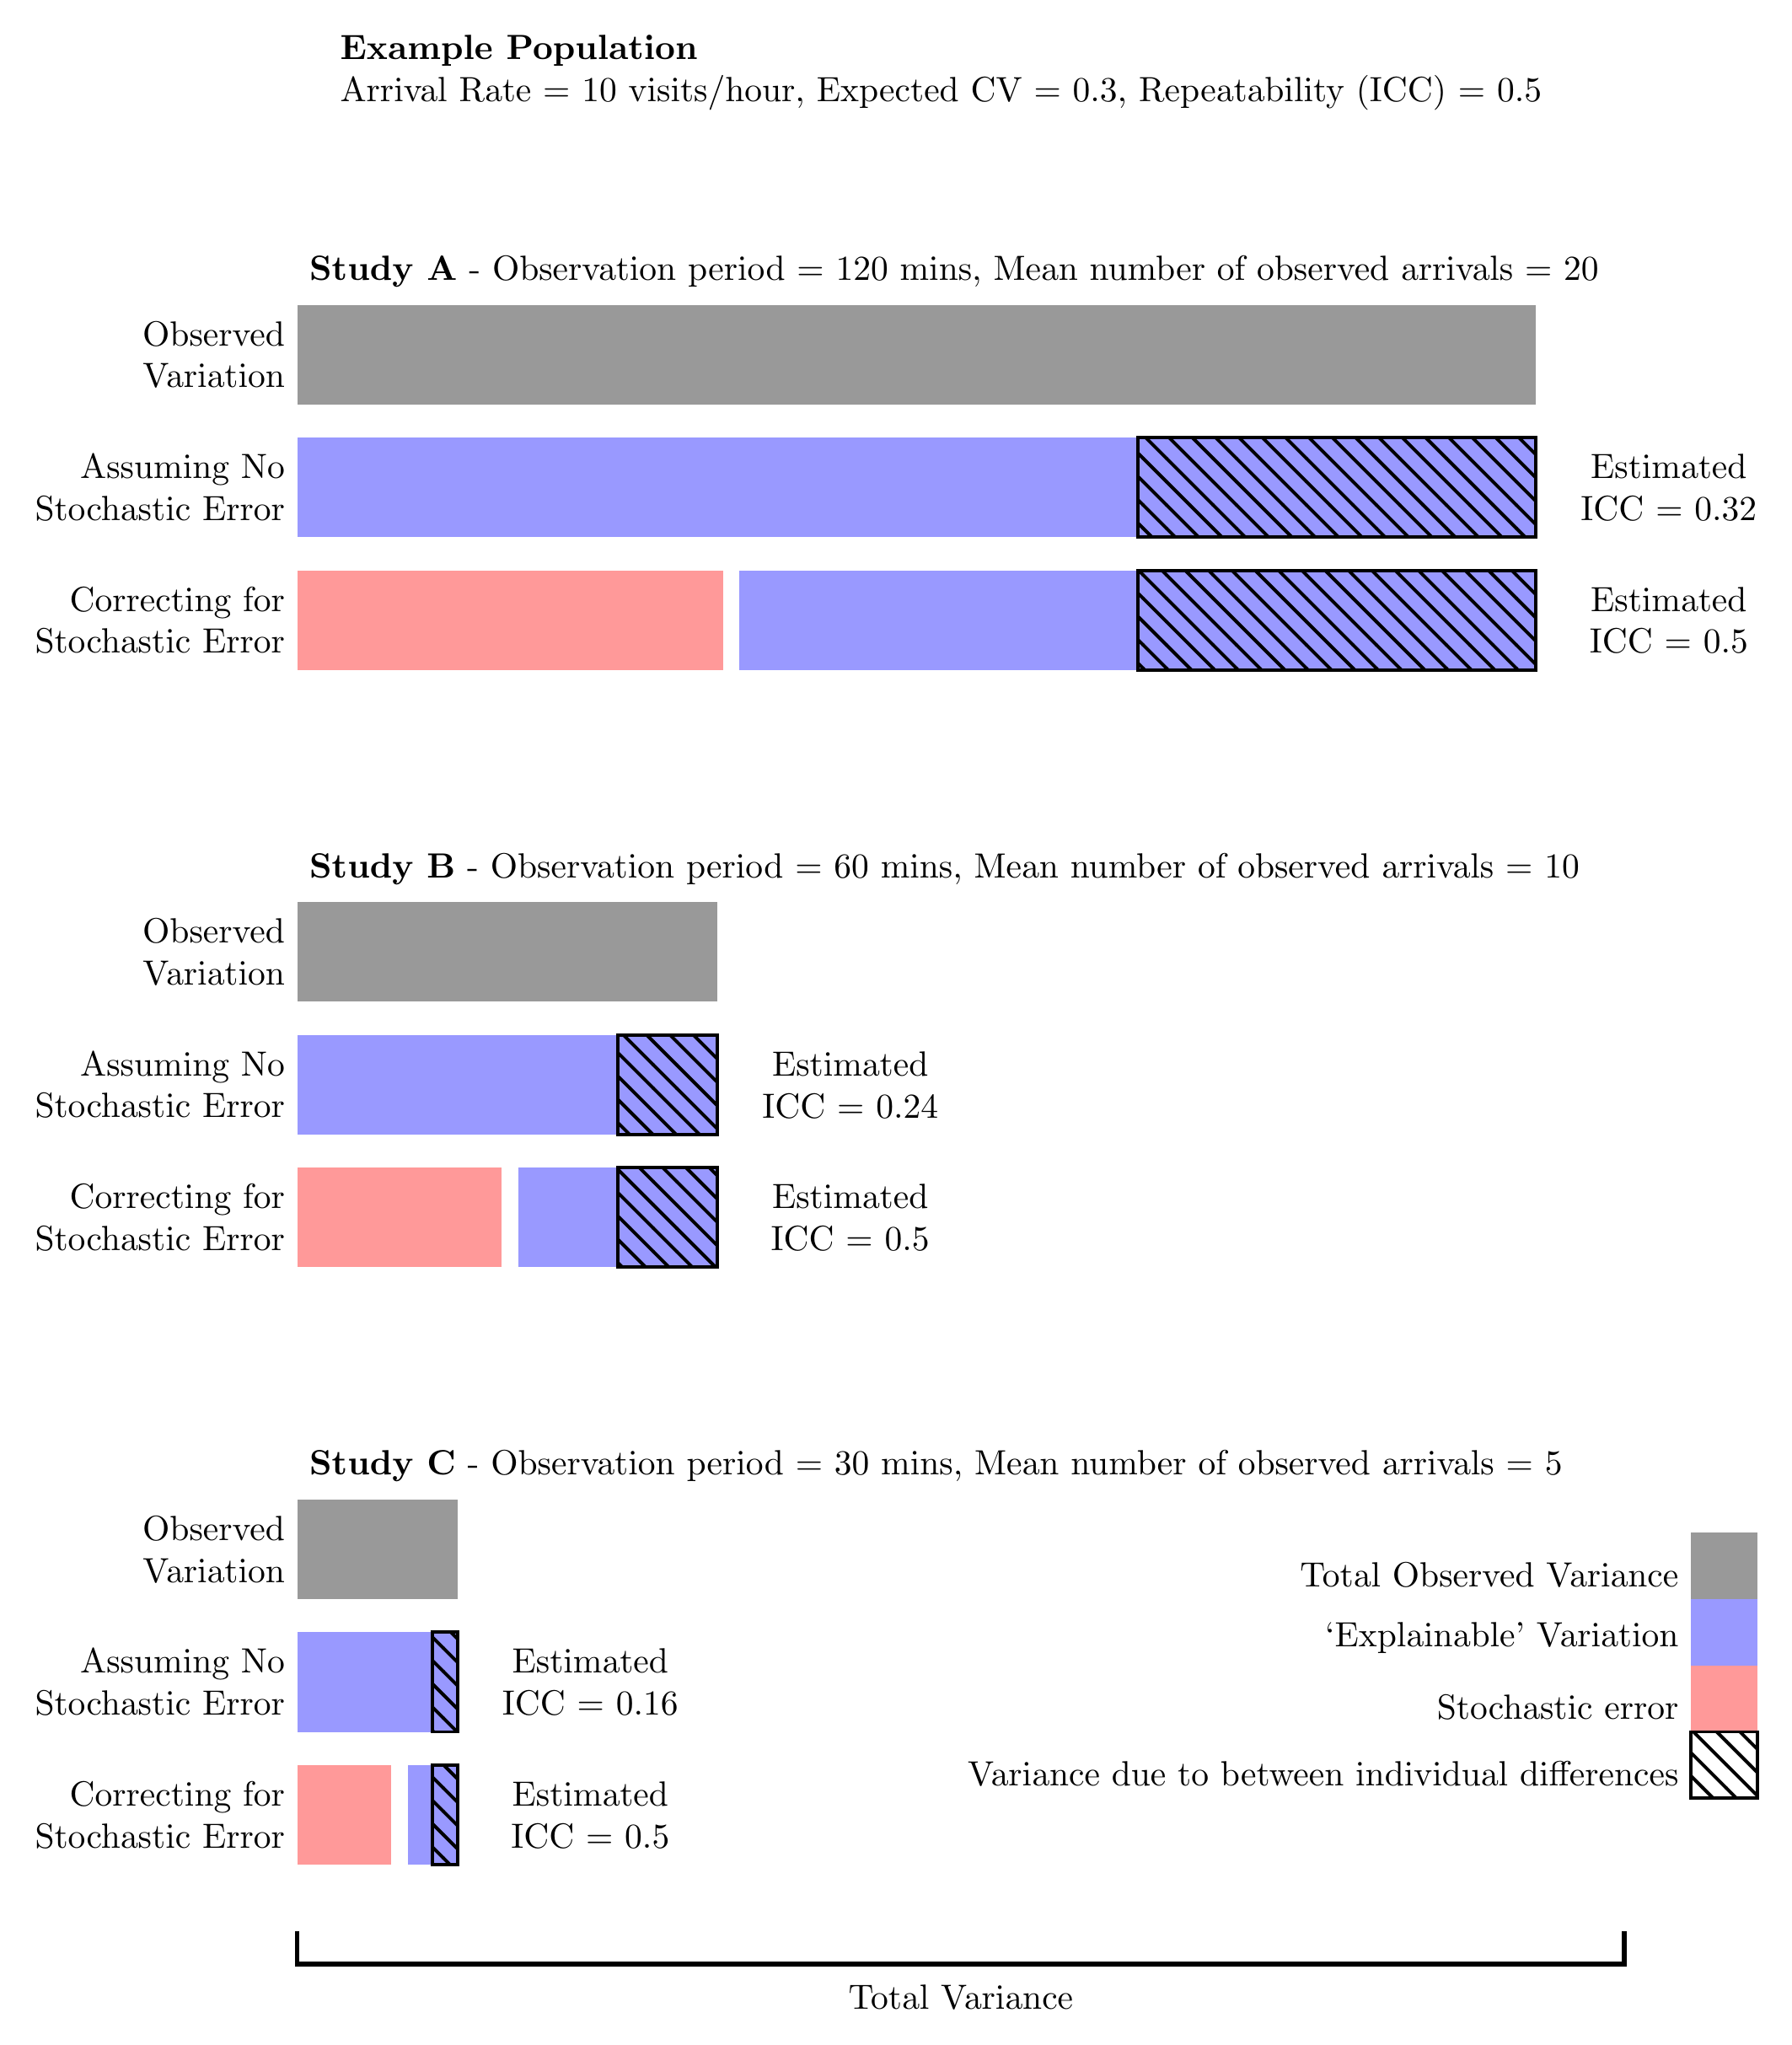
\begin{tikzpicture}[transform shape]

%%%%-------------------------------------------------------------------------------------

\def\scale{3}
\def\cv{0.3}
\def\repeatability{0.5}
\def\rate{10}
\def\exp{(\x *\cv)*(\x*\cv)}
\def\obs{\x +\exp}
\def\x{\rate*\time}


\node[align=left, scale=1.5] at (0.8\textwidth,27) {\textbf {Example Population} \\ Arrival Rate = \rate\ visits/hour,
									Expected CV = \cv, Repeatability (ICC) = \repeatability};


% scale bar
\def\scaleBarY{-1.5}
\draw[line width=0.75mm] (0,\scaleBarY+0.5) -- (0,\scaleBarY) -- (20,\scaleBarY) -- (20,\scaleBarY+0.5);
\node[ scale=1.5] at (10,\scaleBarY-0.5) {Total Variance} ;

% observations time
\def\times{{2,1,0.5}}

% positioning of 'studies'
\def\pos{{18,9,0}}

\def\textarray#1#2{\def#1[##1]{\pgfmatharray{{#2}}{##1}\pgfmathresult}}

\textarray\studies{"A", "B", "C"}




\foreach \i in {0,...,2}{

\pgfmathsetmacro{\time}{\times[\i]}
\pgfmathsetmacro{\y}{\pos[\i]}

% top text
\node[anchor= west, align=left, scale=1.5] at (0,\y+6) {\textbf{Study \studies[\i]} - Observation period = \pgfmathparse{(\time*60)} \pgfmathprintnumber[assume math mode=true]{\pgfmathresult}\ mins, Mean number of observed arrivals = \pgfmathparse{(\time*\rate)} \pgfmathprintnumber[assume math mode=true]{\pgfmathresult}};%


\fill[black!40!white] (0,\y+4) rectangle ({(\obs)/\scale},\y+5.5);
\node[align=right, anchor= east, scale=1.5] at (0,\y+4.75) {Observed \\ Variation} ;

\fill[blue!40!white] (0,\y+2) rectangle ({(\obs)/\scale},\y+3.5);
\draw[pattern=custom north west lines, hatchspread=10pt, hatchthickness=0.5mm, line width=0.5mm]  ({(\obs - (\exp*\repeatability))/\scale},\y+2) rectangle ({(\obs)/\scale},\y+3.5);
\node[align=right, anchor= east, scale=1.5] at (0,\y+2.75) {Assuming No \\ Stochastic Error} ;

\fill[blue!40!white] ({(\x)/\scale},\y) rectangle ({(\obs)/\scale},\y+1.5);
\fill[red!40!white] (0,\y) rectangle ({(\x)/\scale-0.25},\y+1.5);
\draw[pattern=custom north west lines, hatchspread=10pt, hatchthickness=0.5mm, line width=0.5mm] ({(\obs - (\exp*\repeatability))/\scale},\y) rectangle ({(\obs)/\scale},\y+1.5);
\node[align=right, anchor= east, scale=1.5] at (0,\y+0.75) {Correcting for \\ Stochastic Error} ;

\node[align=center, scale=1.5] at ({(\obs)/\scale+2},\y+2.75) {Estimated\\ ICC = \pgfmathparse{(\exp*\repeatability)/(\obs)}%
    \pgfmathprintnumber{\pgfmathresult}};
\node[align=center, scale=1.5] at ({(\obs)/\scale+2},\y+0.75) {Estimated\\ ICC = 0.5};

}


% legend
\def\legx{21}
\def\legy{5}

\fill[black!40!white] (\legx,\legy-1) rectangle (\legx+1,\legy);
\node[anchor=south east, scale=1.5] at (\legx,\legy-1) {Total Observed Variance} ;

\fill[blue!40!white] (\legx,\legy-2) rectangle (\legx+1,\legy-1);
\node[anchor=south east, scale=1.5] at (\legx,\legy-2) {`Explainable' Variation} ;

\fill[red!40!white] (\legx,\legy-3) rectangle (\legx+1,\legy-2);
\node[anchor=south east, scale=1.5] at (\legx,\legy-3) {Stochastic error} ;

\draw[pattern=custom north west lines,hatchspread=10pt, hatchthickness=0.5mm, line width=0.5mm] (\legx,\legy-4) rectangle (\legx+1,\legy-3);
\node[anchor=south east, scale=1.5] at (\legx,\legy-4) {Variance due to between individual differences} ;


\end{tikzpicture}

\end{document}
